\section{DRTA sonda}
    \subsection{Princip fungování}
        \subsubsection{Víceprvková sonda}
    \subsection{Výchozí geometrie}
        Zkoumaná sonda se skládá z dvou odporových teplotní čidel Pt100 (model \textit{1PT100K2515}) o průměru $1.5 \unit{mm}$ a délce $25 \unit{mm}$. Ty jsou umístěny rovnoběžně ve směru proudění pomocí těsnění na jejich koncích, ukotveného v mosazné trubici o průměru $4 \Unit{mm}$ a tloušťce $0.4 \Unit{mm}$, která je využita zároveň k dosažení rozdílu restitučních faktorů jednotlivých čidel. Prostorové uspořádání sestavy je patrné z obrázku \ref{fig:vychozi-DRTA}. Vyšším restitučním faktorem disponuje čidlo umístěné uvnitř trubice a dále v práci o něm bude hovořeno jako o čidlu A. Proudění stíněním čidla A umožňují dva odvětrávací otvory umístěné $12 \Unit{mm}$ od vstupu do trubice. Čidlo umístěné volně v proudícím médiu vykazuje nižší restituční faktor a bude dále značeno jako čidlo B.
        
        \begin{figure}[ht!]
            \centering
            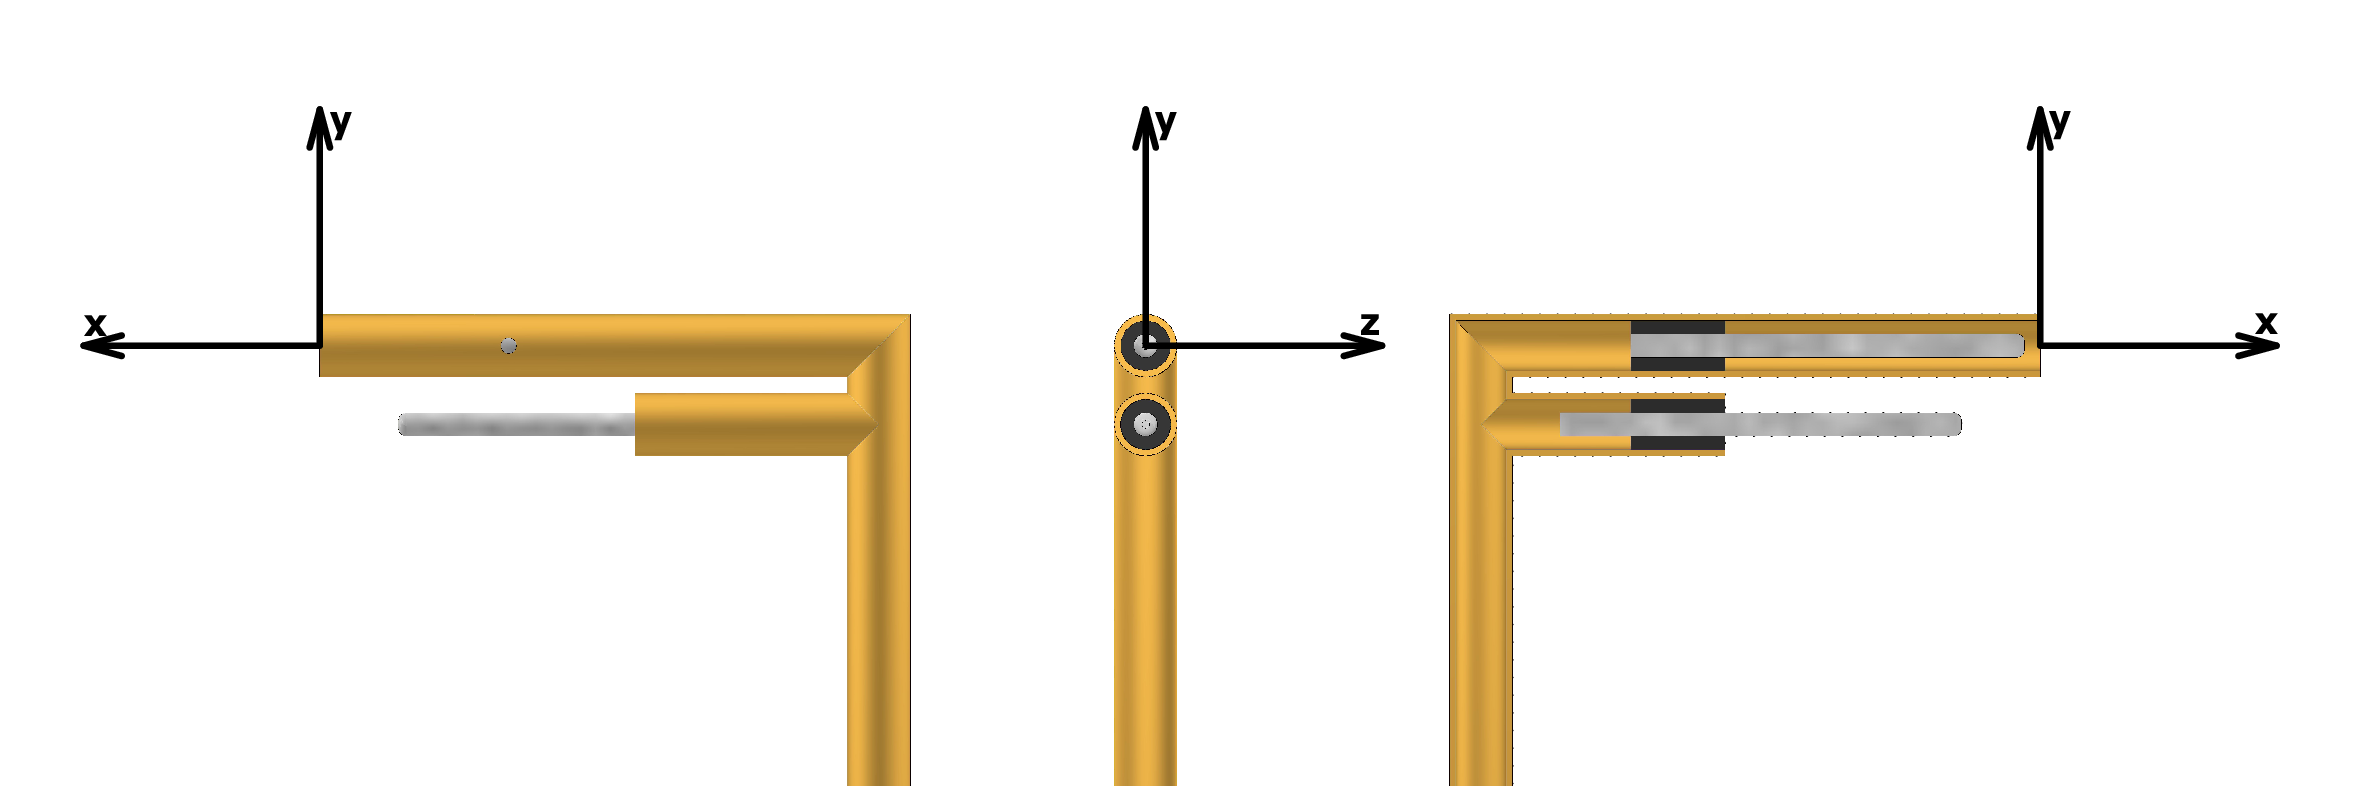
\includegraphics[width=\textwidth]{200_DRTA_SONDA/Vychozi_DRTA.png}
            \caption{Výchozí geometrie DRTA sondy.}
            \label{fig:vychozi-DRTA}
        \end{figure}
    \subsection{Cíle numerických simulací}
        